%%%%%%%%%%%%%%%%%%%%%%%%%%%%%%%%%%%%%%%%%%%%%%%%%%%%%%%%%%%%%%%%%%%%%%
%%  dissertation.tex, to be compiled with latex2e.                   %
%%  Template update 06/01/2024                                       %
%%%%%%%%%%%%%%%%%%%%%%%%%%%%%%%%%%%%%%%%%%%%%%%%%%%%%%%%%%%%%%%%%%%%%%
%%                                                                   %
%%  Writing a Thesis or Dissertation with LaTeX at                   %
%%           Georgia State University                                %
%%                                                                   %
%%  (Running this ``template'' will generate the documentation.)     %
%%                                                                   %
%%%%%%%%%%%%%%%%%%%%%%%%%%%%%%%%%%%%%%%%%%%%%%%%%%%%%%%%%%%%%%%%%%%%%%

\documentclass[12pt,gsu,online]{gsudiss}
% The class file gsudiss.cls is based on the standard report class.
% The body of the text must be in font size either 11pt or 12pt.
% The option 'gsu' is for required line spacing.
% The option 'online' is for the online submission formatting, you should keep this option unless you are preparing a print version of your dissertation.
% You can remove the option "online" to produce a print version which has page number at the center of the footer by default. You can also add one of the options from {'', ''} for customizing the page number location. 

% There is also a draft mode option that can be used to print the word "DRAFT" (or other words defined in the following command) in the header of your dissertation. To enable this option, you can add the option 'drafts' to the class file. Just make sure you disable the "drafts" option before submission.
\printdraft{\textcolor{gray}\small DRAFT}    % In order to use this
                                   % command, you have to enable "drafts"
                                   % in the option of the gsudiss
                                   % class, otherwise it does
                                   % nothing. This prints the word
                                   % "DRAFT" in gray color in the header of your
                                   % dissertation. You can go wild
                                   % here if you want. 


%%%%%%%%%%%%%%%%%%%%%%%%%%%%%%%%%%%%%%%%%%%%%%%%%%%%%%%%%%%%%%%%%%%%%%
% Below is where you include your packages. Add or remove packages as needed.
% There are other packages included in the class file 'gsudiss.cls' that you will not need to add here, including {geometry, calc, ifthen, setspace, tocbibind, tabto, xspace, relsize, color, tocloft, appendix, titlesec, acronym}.

\usepackage{natbib}                % To format bibliographies.
\setlength{\bibsep}{0pt}           % Necessary for bib entries to have
                                   % correct line spacing.

\usepackage[hidelinks]{hyperref}
\hypersetup{colorlinks=false,pdfborder={0 0 0}} % Remove the red boxes around the links

\usepackage{lscape}
\usepackage{array}
\usepackage{deluxetable}
\usepackage{longtable}             % for 'longtable' environment
\usepackage{pdflscape}             % for 'landscape' environment
\usepackage{ltcaption}
% The ltcaption package supports \CaptionLabelFont & \CaptionTextFont
% introduced by the NTG document classes
\renewcommand\CaptionLabelFont{\normalsize}
\renewcommand\CaptionTextFont{\normalsize}

\usepackage[caption = true]{subfig}% for subfigures
\usepackage{amsmath,amsthm,amsfonts,amsopn,amssymb} % Some nice math packages.
\usepackage{eucal}                 % Euler fonts for equations.
\usepackage{verbatim}              % Allows quoting source with commands.
\usepackage{graphicx}              % For powerful manipulation of figures.
\usepackage{ctable}                % My preference table package.
\usepackage[overlay]{textpos}      % Put stuff anywhere, I mean anywhere ...
\usepackage{pstricks}              % Draw stuff especially on top figures etc...
\usepackage{afterpage}             % Useful for absolute placement of figures and tables.
\usepackage{fancyvrb}              % for verbatim environments (see usercommands.tex)

\usepackage{float}
\floatstyle{boxed}
\newfloat{code}{h}{ext}
\floatname{code}{Code}

\usepackage{atbeginend}            % Modify space before and after
                                   % equations. These are my preferences.
\AfterBegin{equation}{\addtolength{\abovedisplayskip}{-0.5\baselineskip}}
\BeforeEnd{equation}{\addtolength{\belowdisplayskip}{-0.5\baselineskip}}
\AfterBegin{equation*}{\addtolength{\abovedisplayskip}{-0.5\baselineskip}}
\BeforeEnd{equation*}{\addtolength{\belowdisplayskip}{-0.5\baselineskip}}

\usepackage{lipsum}                % For generating dummy text in the template.


%%%%%%%%%%%%%%%%%%%%%%%%%%%%%%%%%%%%%%%%%%%%%%%%%%%%%%%%%%%%%%%%%%%%%%
% Below is where you include your thesis/dissertation info.

\author(FirstName LastName) % Your name.

\graduationyear(Year)
\graduationmonth(Month) % The Month and Year here must be the month and year of your graduation—not the month and year of your submission or upload.

\title(Manuscript Title) % The title of your dissertation/thesis.


% Information of your committee members. I have five members as an example below.
% Only the first and last name of your committee members should be listed here. Please do not include their titles. In other words, do not list “Dr.” or “Ph.D.” here. 
\committeeChair(FirstName LastName1) % Committee CHAIR. This has to be non-empty to compile correctly.

\committeeCoChair() % Committee CO-CHAIR. This is useful if you have two advisors. If you do not have a co-chair, you can leave this field empty.

\committee(FirstName LastName2)(FirstName LastName3)(FirstName LastName4)(FirstName LastName5) % Other Committee Members. There has to be at least one to compile correctly. Just add more parentheses for more committee members.


%%%%%%%%%%%%%%%%%%%%%%%%%%%%%%%%
% Custom Options for the table of contents

% You can set the fonts for each section of the TOC using options in the tocloft package
\renewcommand{\cftfigfont}{Figure\ }
\renewcommand{\cfttabfont}{Table\ }
\renewcommand{\cftchapfont}{\bfseries}  % Set the font for the chapters in TOC
\renewcommand{\cftsecfont}{\normalfont} % Set the font for the sections in TOC, e.g., you can change it to \renewcommand{\cftsecfont}{\bfseries}
\renewcommand{\cftsubsecfont}{\itshape}  % Set the font for the subsections in TOC, e.g., you can change it to \renewcommand{\normalfont}
\renewcommand{\cftsubsubsecfont}{\itshape}  % Set the font for the subsubsections in TOC
\renewcommand{\cftparafont}{\mdseries}  % Set the font for the paragraphs in TOC
\setcounter{tocdepth}{2}      % The depth of table of contents, the setting of 2 means it only goes to subsections, you can change it (e.g. 3 is to include subsubsections).


\renewcommand{\topfraction}{0.85}        % These modify figure placement on
\renewcommand{\bottomfraction}{0.85}     % the page and various other space
\renewcommand{\textfraction}{0.10}       % requirements for figures.
\renewcommand{\floatpagefraction}{0.80}  % These 5 lines are not
\renewcommand{\arraystretch}{0.5}        % necessary but I think its better
                                         % than latex default.

\setlength{\tabcolsep}{3pt}        % shrink column spacing so your tables 
                                   % can be wider (yay Todd Tables)
%\setlength{\LTcapwidth}{\textwidth}% so your rotated, normal-sized
                                   % longtable titles won't wrap oddly.


\clubpenalty=1000                  % Make Latex try hard to fix
\widowpenalty=1000                 % "stray lines" in paragraphs,
                                   % i.e. paragraph that begin at the
                                   % last line of a page, or end with
                                   % the last line on the following
                                   % page. This looks silly.
\raggedbottom

\settocname{TABLE OF CONTENTS}              % Set the "Table of Contents"
                                   % name. This is the default. You
                                   % can use "Table of Contents" for example.

\setlofname{LIST OF FIGURES}               % Change the name from 'List of
                                   % Figures'. Use whatever you wish.

\setlotname{LIST OF TABLES}                % Change the name from 'List of
                                   % Tables'. Use whatever suit your
                                   % fancy.

\settocbibname{REFERENCES}         % Change the name from
                                   % 'Bibliography'. Change it back if
                                   % you feel like it.

\setloaname{LIST OF ABBREVIATIONS}
                                   % I Changed the name from 'List of
                                   % Abbreviations'. Use any name that
                                   % makes sense here. If you don't
                                   % have an "abbreviations.tex" file,
                                   % this command will do nothing.

\setfigname{Figure\ }               % Set the caption labels for figures.

\settabname{Table\ }                % Set the caption labels for tables.

\setcapfont{pnc}                   % Set the caption font for
                                   % both tables and figures.

\chapternumsize{\normalsize}            % You can use any standard latex sizes here.
\chapterheadsize{\normalsize}           % You can use any standard latex sizes here.
\chaptertitlesize{\normalsize}           % You can use any standard latex sizes here.
                                   % These defaults look good to me.

\beforechapterheadname{CHAPTER}         % Optional text to put in front of
                                   % the chapter number.
\afterchapterheadname{}          % Optional text to put after the
                                   % chapter number. The default
                                   % looks like this: --1--. Of course
                                   % you can change this to any
                                   % format, for e.g. $\sim$

\chapterheadpos{center}            % You can use 'right', 'left',
                                   % 'center'.

\chaptertitlepos{center}           % You can use 'right', 'left',
                                   % 'center'

\chapterheadverticalspace{-1em}     % The space between the Chapter head
                                   % and the top of page. This distance
                                   % is not absolute, but relative to
                                   % the parameters set by the
                                   % geometry package. Play around
                                   % with this number to suit your needs.

\chapterbetweentitlespace{-1.em}   % The space between the chapter head
                                   % and the title head.

\titleheadverticalspace{2em}       % The space between the title head
                                   % and the text.

\sectiontitlesize{\normalsize}          % This is obvious.
\sectiontitlepos{left}             % Obvious.

\sectiontitleverticalspace{1em}    % The space between the section head
                                   % and the text.

\subsectiontitlesize{\normalsize}       % Obvious.
\subsectiontitlepos{left}          % Obvious.

\subsectiontitleverticalspace{0.5em} % You get the idea...

\subsubsectiontitlesize{\normalsize}
\subsubsectiontitlepos{left}

\subsubsectiontitleverticalspace{0.5em}

\sepabbrev{7em}                    % The space between the abbreviation
                                   % lists, that is, if you have
                                   % one. Has to be >= 5em.

\prettify{pnc}
        % There are many places that's 
                                   % required by the guidelines so
                                   % you can customize. This file
                                   % contains many the options that
                                   % you can set (or just ignore).

\newcommand\arcdeg{\mbox{\ensuremath{^\circ}}}%
\newcommand\arcmin{\mbox{\ensuremath{^\prime}}}%
\newcommand\arcsec{\mbox{\ensuremath{^{\prime\prime}}}}%
\newcommand{\point}{\mbox{\ensuremath{\!\!.}\thinspace}}
\newcommand{\minusone}{\ensuremath{^{-1}}}
\newcommand{\minustwo}{\ensuremath{^{-2}}}
\newcommand{\minusthree}{\ensuremath{^{-3}}}
\newcommand{\minusfive}{\ensuremath{^{-5}}}
\newcommand{\plusthree}{\ensuremath{^{3}}}
\newcommand{\plusfive}{\ensuremath{^{5}}}
\newcommand{\kms}{\mbox{\ km\,s\ensuremath{^{-1}}}}
\newcommand{\fig}{Figure~}
\newcommand{\figs}{Figures~}
\newcommand{\tab}{Table~}
\newcommand{\tabs}{Tables~}
\newcommand{\eqn}{Equation~}
\newcommand{\eqns}{Equations~}
\newcommand{\vracc}{\mbox{$\mathrm{v=kr}$}\xspace}
\newcommand{\vrdec}{\mbox{$\mathrm{v=v_{max}-k^{'}(r-r_t)}$}\xspace}
\newcommand{\vrootracc}{\mbox{$\mathrm{v=k_{1}\sqrt r}$}\xspace}
\newcommand{\vrootrdec}{\mbox{$\mathrm{v=v_{max}-k_{2}\sqrt{r-r_t}}$}\xspace}
\newcommand{\rlaw}{\mbox{$r\ $law}\xspace}
\newcommand{\rootrlaw}{\mbox{$\sqrt r\ $law}\xspace}
\newcommand{\resolvingpower}{\mbox{$\lambda/\Delta\lambda$}\xspace}
\newcommand{\OIII}{\mbox{[\acs{O3}]}\xspace}
\newcommand{\solarmass}{\mbox{\ M\ensuremath{_{\odot}}}}
\newcommand{\arcpt}{${{\lower3pt\hbox{$^{\prime\prime}$}}\atop{\raise4pt\hbox{.}}}$}
\newcommand{\msun}{$M_\odot$}               % You can put some self-defined
                                   % commands in this file like
                                   % math command abbreviations, etc.


%%%%%%%%%%%%%%%%%%%%%%%%%%%%%%%%%%%%%%%%%%%%%%%%%%%%%%%%%%%%%%%%%%%%%%
%                 The document starts here.                          %
%%%%%%%%%%%%%%%%%%%%%%%%%%%%%%%%%%%%%%%%%%%%%%%%%%%%%%%%%%%%%%%%%%%%%%
\begin{document}

%%%%%%%%%%%%% The front matter of your document %%%%%%%%%%%%

% Tile and abstract pages are required. To edit your title and abstract pages, go to `./FrontMatters/TitleAbstract.tex' file.
\pagestyle{empty}
\begin{center}
Manuscript Title % Your title should be in title caps.

%%%%%%%%%%%%%%%%
% If it takes more than two lines, it must be double-spaced, for example,

% Manuscript Title line 1
% \vspace*{.1in}
% Manuscript Title line 2
%%%%%%%%%%%%%%%%

\vspace{1.4in}
by\\
\vspace{1.4in}
First and Last Name\\ %Your name should be in title caps.
\vspace{1.4in}
Under the Direction of Committee Chair's Name, MA/Ph.D. \\ %List your supervisor's first and last name followed by their letter credentials. Do not put their title before their name.
\vspace{1.4in}
A Thesis/Dissertation Submitted in Partial Fulfillment of the Requirements for the Degree of\\  % Choose either thesis or dissertation and delete the other.
\vspace{.2in}
Level and Degree Title \\ % Your degree does not include your specialization. The following are your options: Master of Arts, Master of Science, or Doctor of Philosophy. Do NOT list your department/field here.
\vspace{.2in}
in the College of Arts and Sciences \\
\vspace{.2in}
Georgia State University \\
\vspace{.2in}
Year

\end{center}

\pagebreak 


\begin{center}
    ABSTRACT\\ 
\end{center}

\doublespacing
The abstract paragraph is mandatory. Start the abstract paragraph here. Double-space this paragraph. Limit the abstract of a thesis to 150 words. Limit the abstract of a dissertation to 350 words. ``Your abstract will not be accepted if it exceeds the limit by even one word.''

\begin{singlespace}
\vfill   
\vspace{0.5in}
\noindent INDEX WORDS:
\hspace{0in}
\parbox[t]{4.5in}{
Sample keyword, Sample keyword, Sample keyword}  %It is recommended that you list six keywords. Please use my capitalization here as an example. Should be single-spaced.
\end{singlespace} 

\frontmatter % This line is supposed to be here.

% The copyright page is required. To edit your name and year, please go to \author()
\copyrightpage

% The approval page is required. To edit the committee and other information, please go to \committeeChair(), \committeeCoChair(), \committee(), etc.
\approvalpage

% The dedication page is optional. You can write your dedication in `./FrontMatters/dedication.tex' file. Delete that file if you don't want to include it. This command does nothing if you don't have a `dedication.tex' file.
\dedicationpage

% The acknowledgment page is optional. You can write your acknowledgment in `./FrontMatters/acknowledgment.tex' file. Delete that file if you don't want to include it. This command does nothing if you don't have an `acknowledgment.tex' file.
\acknowledgmentpage

% Table of Contents will be automatically generated and placed here.
\tableofcontents

% List of Tables will be automatically generated if you had made proper table captions.
\listoftables

% List of Figures will be automatically generated if you had made proper figure captions.
\listoffigures

% The list of abbreviations is optional. List of Abbreviations will be automatically generated if you had made any in `./FrontMatters/abbreviations.tex' file following the style of the "Acronym". See that file for example usage. Delete that file if you don't want to include it. This command does nothing if you don't have an `abbreviations.tex' file.
\listofabbreviations


%%%%%%%%%%%%%%%%%%%% The main chapters %%%%%%%%%%%%%%%%%%%%%

\pagestyle{plain}

\mainmatter                        % Main chapters starts here

% The chapter order is determined by the order of the \include commands below.
% Edit the chapter contents in the respective files in the `./Chapters/` directory. You can add more chapters by adding more files and more \include commands below.
\chapter{Introduction}
\label{chap:introduction}

\section{Your Section Title Here}
	You should probably introduce some stuff here.

\subsection{Your Subsection Title Here}
You should probably introduce some stuff here.

You should look at the gsudiss.cls file first when you want to change things in how the document is laid out. 

You can refer to your other chapters like this: \chap\ref{chap:chapter_2}. Since Appendix is not numbered, you can refer to it like this: \hyperref[chap:appendix]{Appendix}.

\subsubsection{Your Subsubsection Title Here}
This is the content for the subsubsection.

\chapter{Example Chapter Title}
\label{chap:example_chapter}

This is an example chapter with some text. You don't need to name your chapters as "Chapter 1", "Chapter 2", etc. Rather, following the practice of \LaTeX, it is better to name and label your chapters descriptively. And the numbering of the chapters will be done automatically when you include them in your \verb|main.tex| file. If you want to include a new chapter in your document, create a \verb|chapter_name.tex| file in the \verb|Chapters| directory and include it in your \verb|main.tex| file using the \verb|\include{./Chapters/chapter_name}| command.

You can include figures, tables, and equations in your chapters. You can also include subfigures and subtables. I selected a few texts in the formatting guidelines and provided some examples below.

\section{Headings and Subheadings}
\label{sec:headings}

Graduate Services does not set specific style standards for the format of chapter headings and subheadings except for font size—font size for all headings should be the same as the body of your text (if your text is 12 pt., then your headings must also be 12 pt.). There is a suggested format for heading style in the required templates provided by Graduate Services. Students should refer to the standards set by their department's choice of style manual. Regardless of the formatting style chosen, Graduate Services does require that the style be applied consistently to all headings and subheadings throughout the document. 


\section{Journal Articles Used as Chapters}
\label{sec:journal_articles}
In some departments, theses or dissertations may include as chapters, articles that have been or will be submitted to scholarly journals. This is an acceptable style; however, you must be listed as an author with clear evidence of your intellectual leadership in the publication. How this is represented varies across disciplines; it may take the form of sole authorship, lead authorship, or corresponding authorship, and the publication may not be included in any other individual's thesis or dissertation, whether at GSU or any other institution. A brief statement should be included at the conclusion of the chapter describing the intellectual leadership and any other research roles played by the student in developing and publishing the research. 
 
In addition, the general formatting requirements listed above also apply to articles used as chapters. You MUST apply a consistent style in your font, headings, subheadings, tables and figures throughout each article used as a chapter, as well as your general introduction and conclusion. Evidence of permission to use articles which have been published or accepted for publication must be included. It is the student's responsibility to secure such copyright releases prior to submitting the thesis/dissertation to Graduate Services. Graduate Services will accept a letter of permission or an e-mail from the publisher. Graduate Services will not accept a thesis or dissertation for the final submission unless all copyright releases are on file (articles that have yet to be submitted or are under review do not need copyright releases.) 





\section{Reference Examples}
\label{sec:reference_examples}

And as an example of citing things, here is the \TeX book by Knuth in 1986~\cite{knuth1986texbook}. See \verb|bibliography.bib| for adding reference items. Format of the reference entries should be according to your department or discipline's choice of style manual. That said, you do have the option to create references or works cited pages for each chapter rather than a large comprehensive list of references.


\section{Figures and Tables}
\label{sec:figures_tables}

Sample Figures and Tables below.

\begin{figure*}[H]
	\centering
	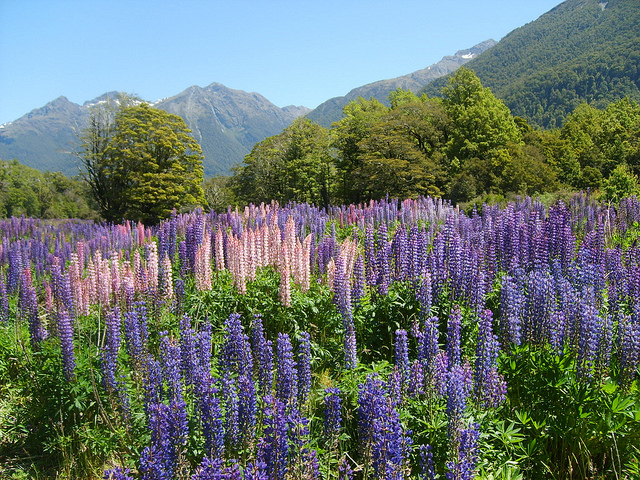
\includegraphics[width=0.7\textwidth]{./Plots/nature.jpg}
	\caption{An individual figure!}
\end{figure*}
        
\begin{figure*}[H]
	\centering
	\subfloat[\label{fig:HD8538_ellplot}]{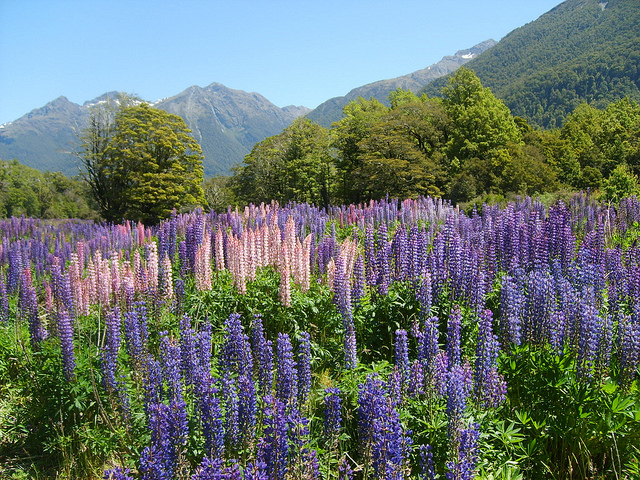
\includegraphics[width=.4\textwidth]{./Plots/nature.jpg}} 
	\subfloat[\label{fig:HD8538_phot}]{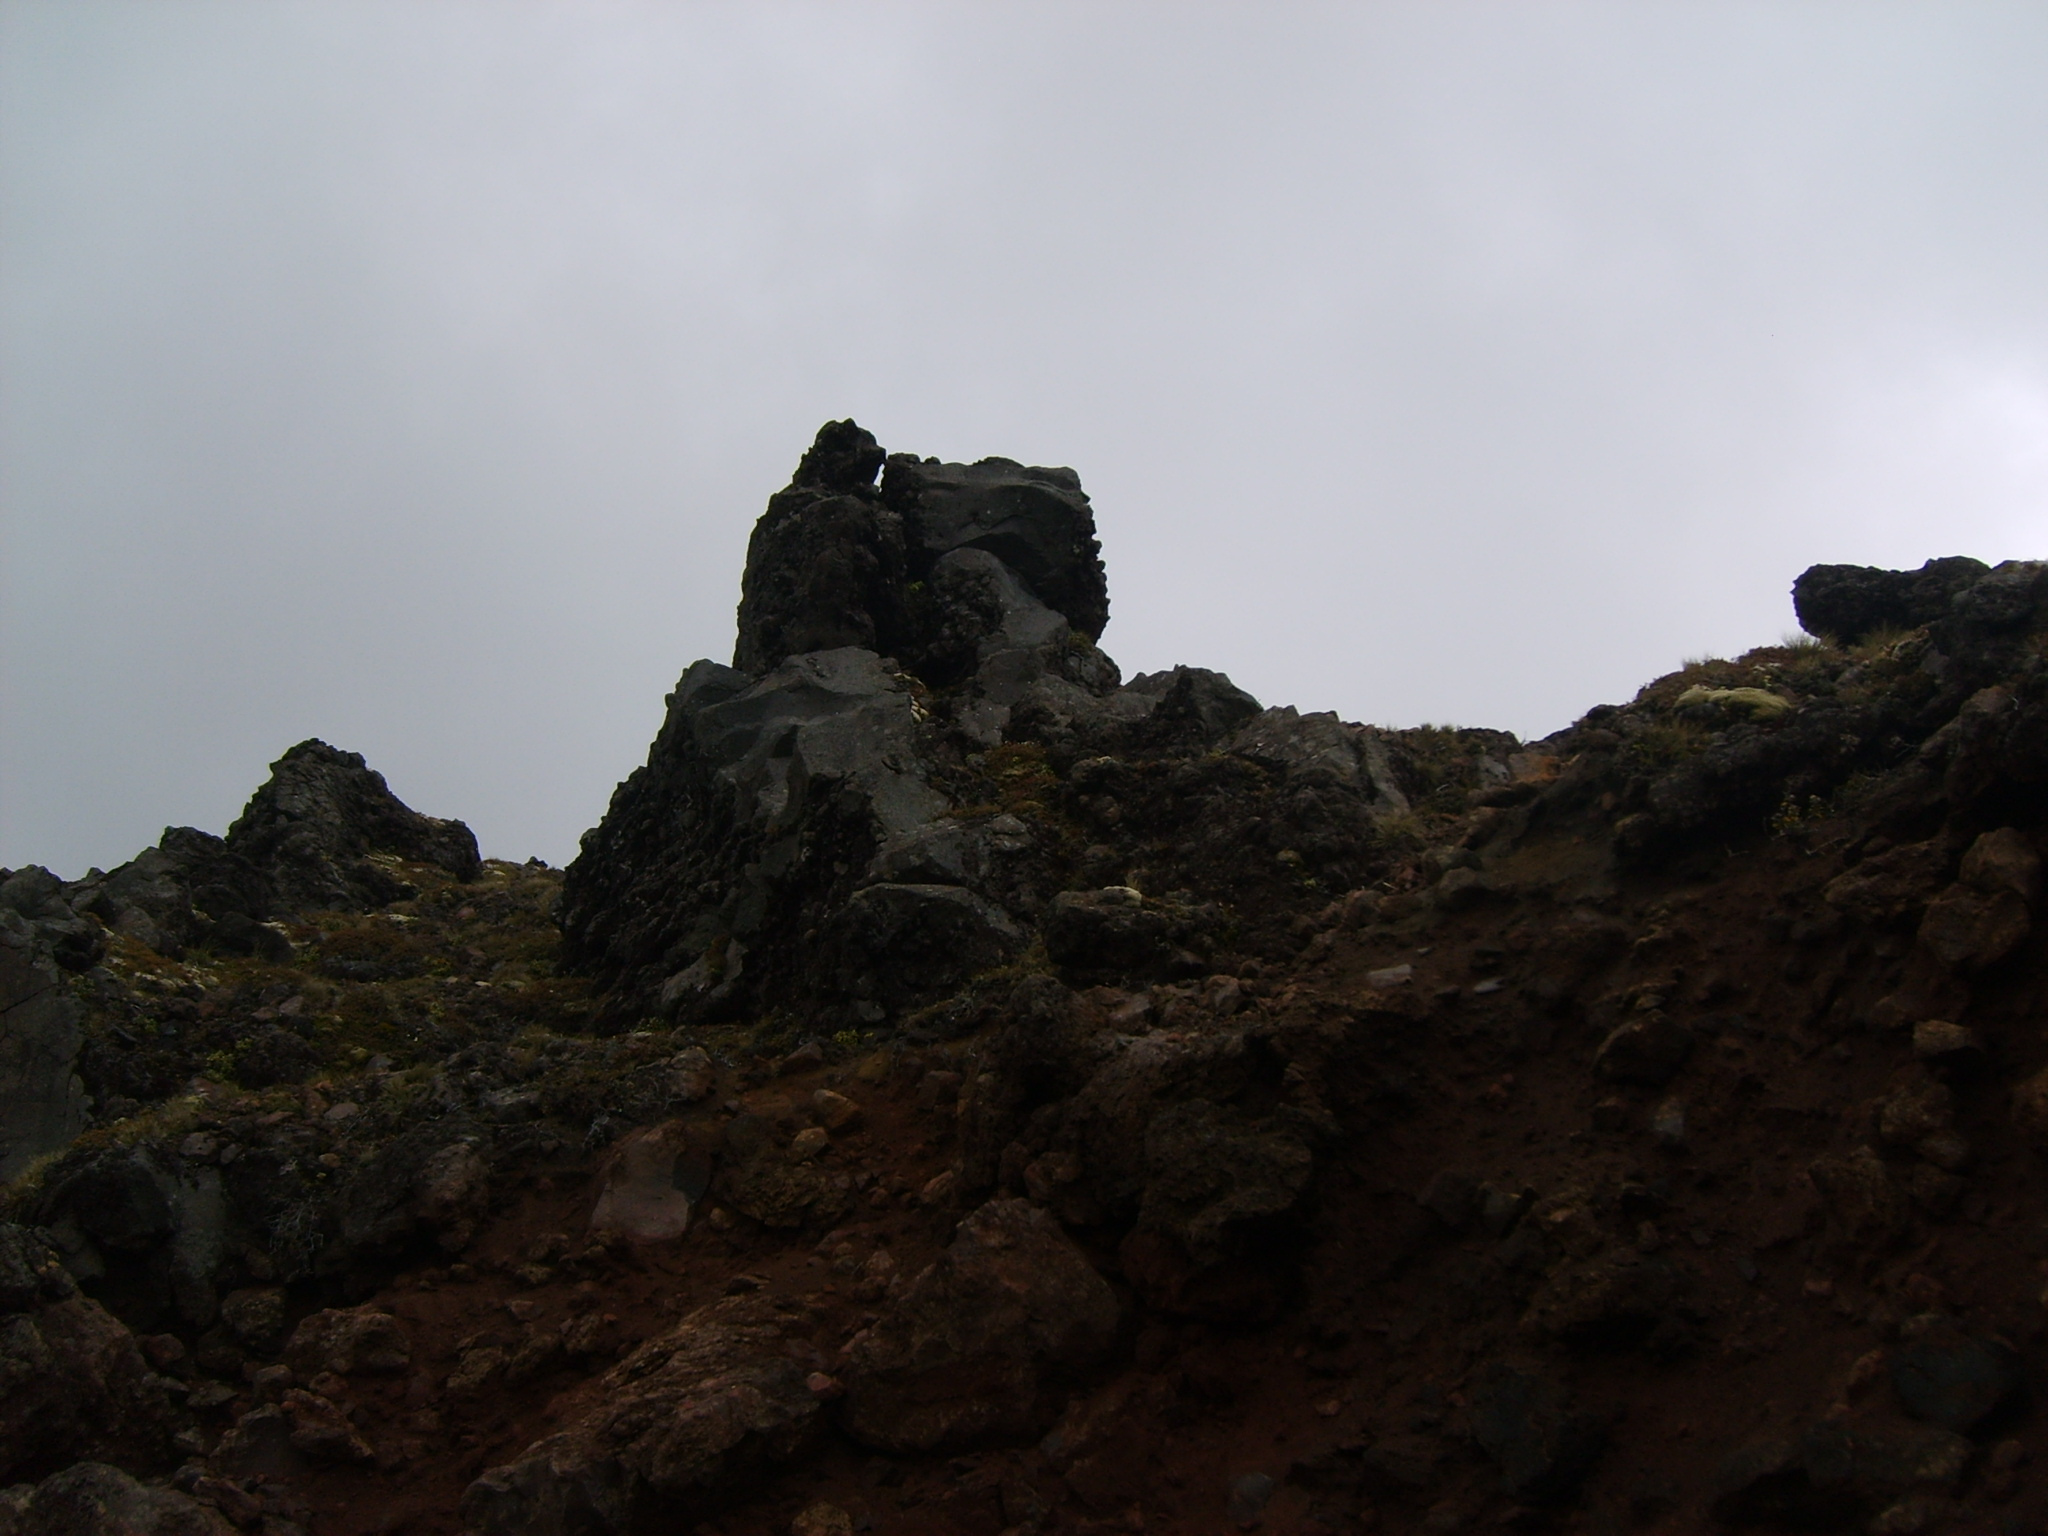
\includegraphics[width=.4\textwidth]{./Plots/rocks.jpg}} \\
	\subfloat[\label{fig:HD8538_vis}]{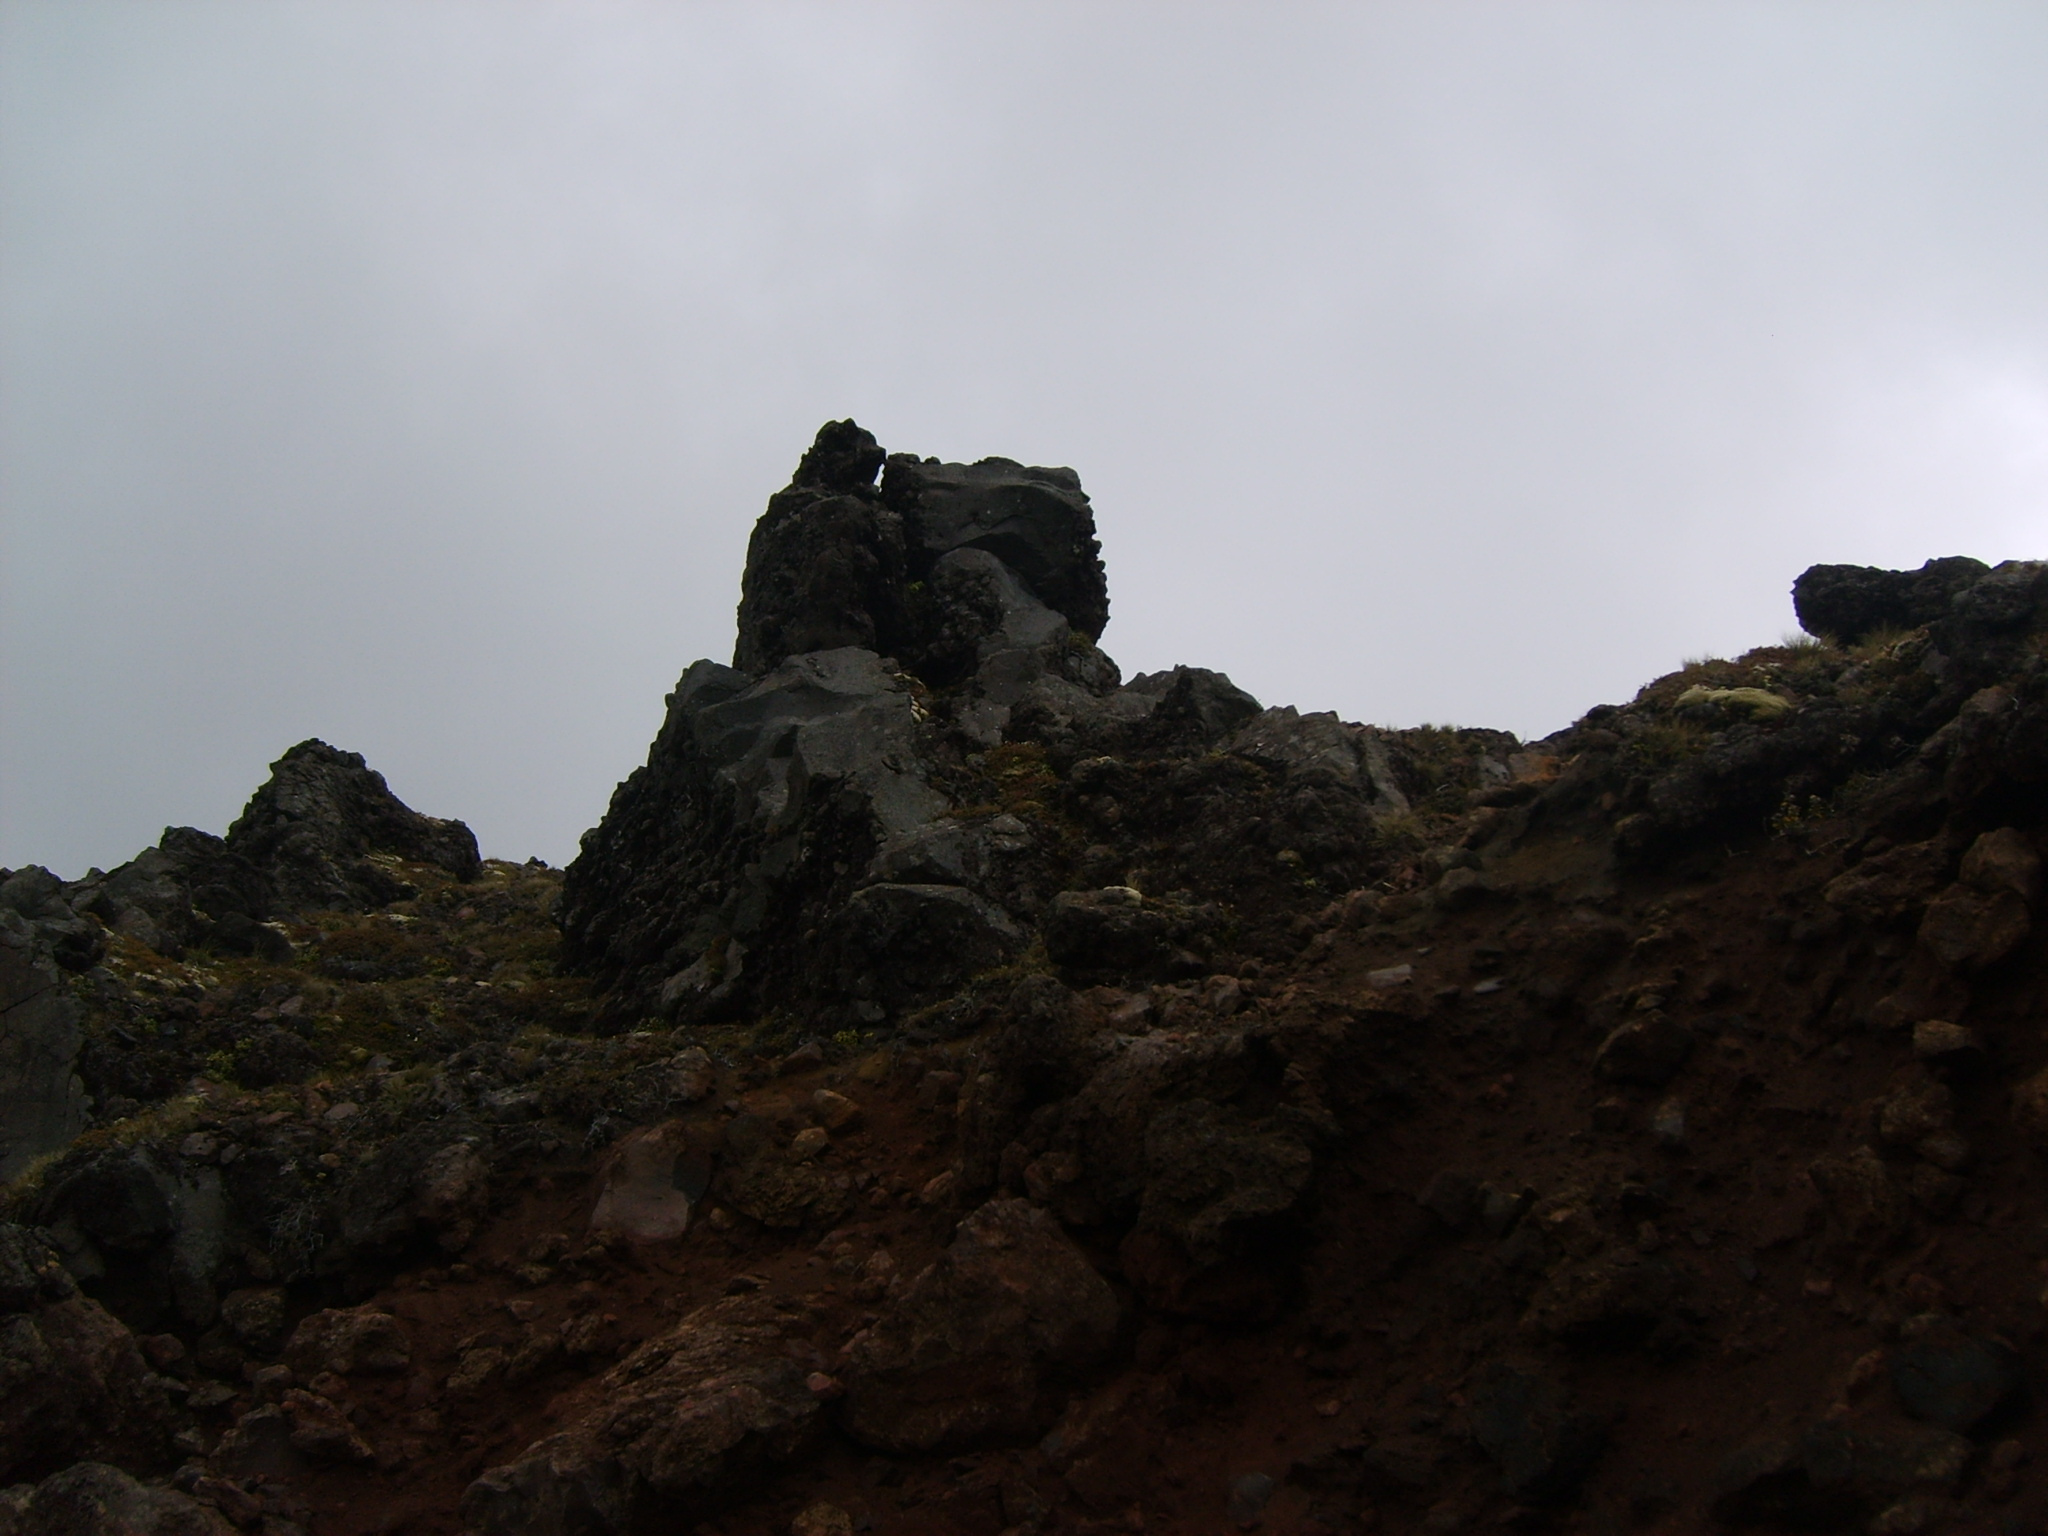
\includegraphics[width=.4\textwidth]{./Plots/rocks.jpg}}
	\subfloat[\label{fig:HD8538_HRD}]{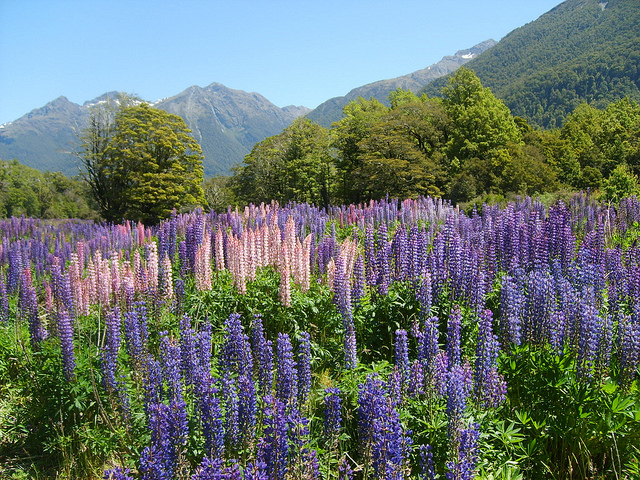
\includegraphics[width=.4\textwidth]{./Plots/nature.jpg}}
	\caption{Multiple figures!}
\end{figure*}

You can have a table like this:
\begin{table}[H]
	\centering
	\label{tab:simple_table}
	\caption{A simple table}
	\begin{tabular}{|c|c|c|}
		\hline
		\textbf{ID} & \textbf{Name} & \textbf{Course} \\
		\hline
		1 & John Doe & Mathematics \\
		2 & Jane Smith & Physics \\
		3 & Mary Johnson & Chemistry \\
		\hline
	\end{tabular}
\end{table}

You can also include a wide table like this:

\begin{landscape}
\begin{longtable}{cccccccccccccc}
\label{tab:wide_table_example}\\
\caption{An example of very large horizontal table}\\
\hline\endhead  % header material
\hline\endfoot  % footer material
\hline
\textbf{ID} & \textbf{Name} & \textbf{Age} & \textbf{Email} & \textbf{Phone} & \textbf{Major} & \textbf{Grade} & \textbf{Comments} \\
\hline
1 & John Doe & 20 & johndoe@example.com & 123-456-7890 & Mathematics & A & Excellent work \\

2 & Jane Smith & 22 & janesmith@example.com & 234-567-8901 & Physics & B & Good understanding \\

3 & Mary Johnson & 21 & maryjohnson@example.com & 345-678-9012 & Chemistry & A & Outstanding performance \\

4 & James Brown & 23 & jamesbrown@example.com & 456-789-0123 & Biology & C & Needs improvement \\

5 & Patricia Davis & 20 & patriciadavis@example.com & 567-890-1234 & English & B & Well done \\

6 & Robert Miller & 22 & robertmiller@example.com & 678-901-2345 & History & A & Excellent analysis \\

7 & Jennifer Wilson & 21 & jenniferwilson@example.com & 789-012-3456 & Geography & B & Good research \\

8 & Michael Moore & 23 & michaelmoore@example.com & 890-123-4567 & Computer Science & A & Great coding skills \\

9 & Linda Taylor & 20 & lindataylor@example.com & 901-234-5678 & Art & C & More practice needed \\

10 & William Anderson & 22 & williamanderson@example.com & 012-345-6789 & Music & B & Good performance \\
\hline
\end{longtable}
\end{landscape}


\section{Examples and Code Snippets}

Here is an example of code snippet:
\begin{code}
	print("Hello World!")
	for i in range(10):
		print(i)
\end{code}

If you want some example text, here is some:
\begin{example}
	Your example here
\end{example}


%%%%%%%%%%%%%%%%%%%% The back matters %%%%%%%%%%%%%%%%%%%%%%

\appendix

% Choose one of the following two options. If you have only one appendix, use the first option. If you have more than one appendices, use the second option. Edit the appendix contents in the respective files in the `./BackMatters/` directory.
% Use this file if you have only one appendices. If you have more than one appendix, use Appendices.tex instead
% If you want to write multiple sections in the appendix, it's better also use Appendices.tex 

\chapter*{APPENDIX}
\label{chap:appendix}
\addcontentsline{toc}{chapter}{APPENDIX}

This is the appendix! You can actually have a ``phantom'' section in the appendix like the following and refer to it in your text like this: \hyperref[sec:appendix_phantom_section]{Appendix}.

\phantomsection
\section*{A section title in the appendix}
\label{sec:appendix_phantom_section}

However, you probably want to use \verb|Appendices.tex| instead of this file if you really have multiple appendices instead of separating phantom sections.

% % Use this file if you have more than one appendices. If you have only one appendix, use Appendix.tex instead.

\chapter*{APPENDICES}
\addcontentsline{toc}{chapter}{APPENDICES}

\section{Something}
This is the appendix!

\subsection{First subsection}
Explain some more details here.


\section{Something Else}
Another appendix!


% The bibliography starts here. Please learn to use the formatting of Latex's Bibtex. It is very powerful and will make your life easier.
% Format the entries according to your department or discipline’s choice of style manual.
% "mybibliography.bib" contains some Bibtex item examples.
\bibliographystyle{plain}
\bibliography{mybibliography}


\end{document}
%%%%%%%%%%%%%%%%%%%%%%%%%%%%%%%%%%%%%%%%%%%%%%%%%%%%%%%%%%%%%%%%%%%%%%
%                  The document ends here.                           %
%%%%%%%%%%%%%%%%%%%%%%%%%%%%%%%%%%%%%%%%%%%%%%%%%%%%%%%%%%%%%%%%%%%%%%
